\section{PS1: Photomagic with LFSR}\label{sec:ps1}

\subsection{Overview}\label{sec:ps1:overview} % A discussion of the assignment itself

In this project, we were tasked with making a program that could encrypt and decrypt an image given a binary seed.
To do this, a class FibLFSR was made with similarities to a linear feedback shift register.
Using this class, an image's pixels could be randomized and the image could be 'encrypted'.  
Based off the design of the FibLFSR, an image could be encrypted and decrypted given the same seed was used.

\subsection{End Product}\label{sec:ps1:accomplish} % What I accomplished and images/results

Below is the output.
On the left is the encryption, from the Darth Vader image into seeming random 'static'.
On the right is the decryption, from 'static' back into the original Darth Vader image.

\begin{figure}[h]
\centering
\begin{minipage}[b]{0.4\textwidth}
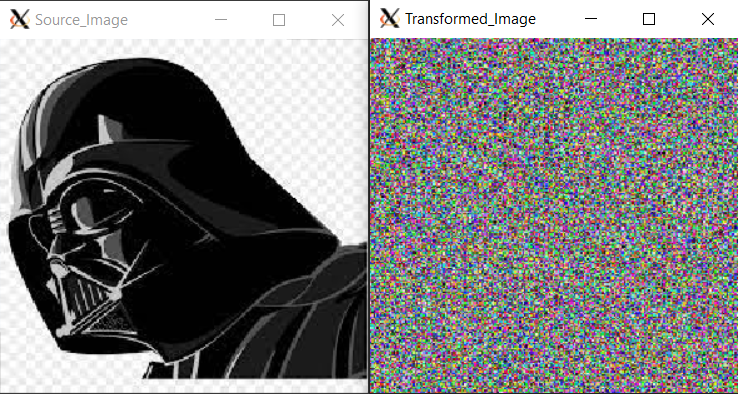
\includegraphics[width=\textwidth]{ps1-1_output}
\caption{Encryption}
\end{minipage}
\hfill
\begin{minipage}[b]{0.4\textwidth}
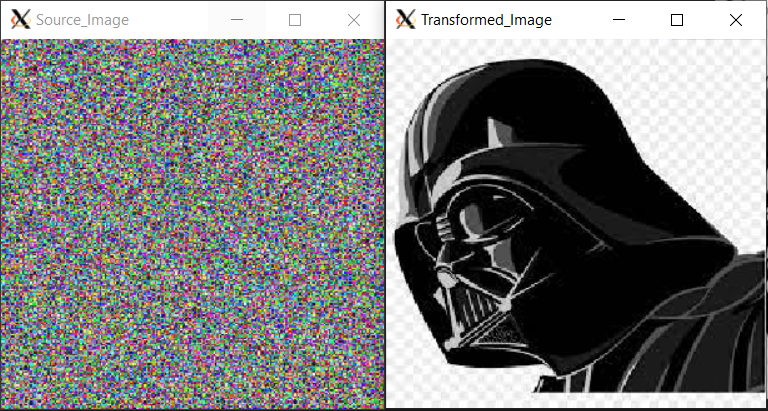
\includegraphics[width=\textwidth]{ps1-2_output}
\caption{Decryption}
\end{minipage}
\end{figure}

\subsection{What I Already Knew}\label{sec:ps1:knew} % What was known prior to the assignment

I knew how to shift bits and how shift registers worked for reference when creating the LibLFSR class.
I also knew how to make a window and draw to it in SFML from ps0.

\subsection{Design Decisions and Implementations}\label{sec:ps1:decisions} % Important decisions or implementations I made

I chose to represent the FibLFSR class as a string. 
This made it so accessing certain elements and appending or taking a character from the front to represent a shift wasn't too difficult.
Inside the class, the 'step' function was made to represent a shift.
This function XORed specific bit positions, with the final bit result being appended to the string, and the front bit being removed.
This was then used by 'generate' function to make a binary number of a given size.
The function looped for a given size and generated a bit until it had a string of bits and had created a number.
To encrypt/decrypt the image, the 'transform' function used this idea to randomize a given image's pixels.
Each pixel's rgb value could be represented as an 8-bit number so 'generate' was used with an argument of 8 to seemingly generate a completely random red, green, or blue value.
This made each pixel completely different from it's original rgb values.
\bigskip

As extra credit I made it so not only a binary seed could be used to encrypt the image, but a seed of any numbers or characters could be used.
For this, I accounted for any character located in the ASCII table.
What I did was make any odd characters in the ASCII table a 1 and any even a 0.
This made it so 0 and 1 still remained the same while other characters could now be made into 0s and 1s.
Any password over length 16 had those trailing bits ignored and anything shorter had it's remaining bits alternating between '0's and '1's.
These together make it seem as random as possible while also making it so the same alphanumeric seed made the same binary seed every time.

\subsection{What I Learned}\label{sec:ps1:learned} % What I learned because of the assignment

I learned how to run two windows simultaneously in SFML.
For an image, I learned how access and edit the rgb values of it's pixels.

\subsection{Challenges}\label{sec:ps1:challenges} % Challenges along the way and any that went unresolved

There were were no major complications along the way.

\newpage
\subsection{Codebase}\label{sec:ps1:code} % Code: Makefile, .cpp main, .hpp main, .cpp support, .hpp support, .cpp tests

\bigskip
\title{\large Makefile:}
\lstinputlisting{../ps1b/Makefile}
\bigskip
\title{\large Photomagic.cpp:}
\lstinputlisting{../ps1b/Photomagic.cpp}
\bigskip
\title{\large FibLFSR.cpp:}
\lstinputlisting{../ps1b/FibLFSR.cpp}
\bigskip
\title{\large FibLFSR.hpp:}
\lstinputlisting{../ps1b/FibLFSR.hpp}
\bigskip
\title{\large test.cpp:}
\lstinputlisting{../ps1b/test.cpp}

\newpage


